\documentclass[border=2pt,12pt]{standalone}
\usepackage{tikz}
\usetikzlibrary{positioning}

\begin{document}
\pagestyle{empty}

\begin{tikzpicture}
%[scale=1,every node/.style={minimum size=0.5cm},on grid]
    \begin{scope}
            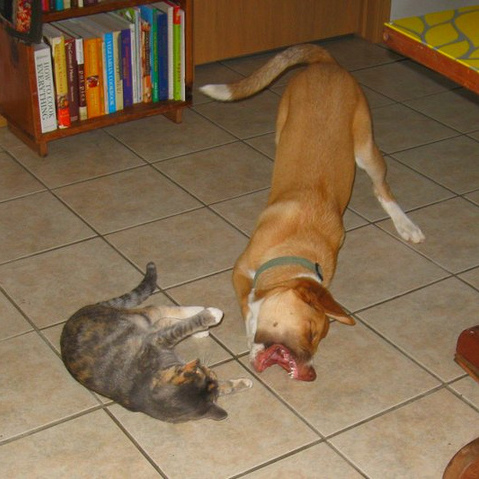
\includegraphics[width=0.25\linewidth]{ILSVRC2014_train_00047188_479x479.JPEG}
    \end{scope}
    \begin{scope}
            %\draw[xshift=0.35mm,yshift=0.35mm,step=10mm, black, thin] (0,0) grid (8,8);
        \draw[xshift=0.35mm,yshift=0.35mm,step=10mm, black, thin] (0,0) grid (0,0);
        \draw[blue,  thick] (0.41, 0.38) rectangle (1.80, 1.59);
        \draw[red,  thick] (1.42, 0.69) rectangle (3.10, 3.15);
    \end{scope}
    \draw[](1.5, 0) node[below, align=center]{\scriptsize (a) Input image with GT boxes};
        
    \begin{scope}[xshift=36mm]
       \draw[step=4.3mm, black] (0, 0) grid (3.44,3.44);
                 \draw[black, dashed] (0.93,0.93) rectangle (1.23,1.23);
            \draw[blue, dashed,  thick] (0.67,0.67) rectangle (1.49,1.49);
            \draw[blue, dashed,  thick] (0.52,0.78) rectangle (1.64,1.38);
            \draw[black, dashed] (0.78,0.52) rectangle (1.38,1.64);
            
            \draw[black, dashed] (2.22,1.78) rectangle (2.52,2.09);
            \draw[black, dashed] (1.96,1.53) rectangle (2.78,2.35);
            \draw[black, dashed] (1.81,1.64) rectangle (2.93,2.24);
            \draw[black, dashed] (2.07,1.38) rectangle (2.67,2.5);
    \end{scope}
    \draw[](5.4, 0) node[below]{\footnotesize (b) $8\times 8$ feature map};
      
    \begin{scope}[xshift=72mm]
       \draw[step=8.6mm, black] (0,0) grid (3.44,3.44);
             \draw[black, thick] (1.72,1.72) rectangle (2.59,2.59);
            \draw[black, dashed] (1.85,1.85) rectangle (2.46,2.46);
            \draw[black, dashed] (1.34,1.34) rectangle (2.97,2.97);
            \draw[black, dashed] (1.03,1.55) rectangle (3.28,2.76);
            \draw[red, dashed, ultra thick] (1.55,1.03) rectangle (2.76,3.28);
            \fill[nearly opaque, white] (0.1, 0.01) rectangle (3,0.85);
    \end{scope}
    \draw[](9, 0) node[below]{\footnotesize (c) $4\times 4$ feature map};
 
    \draw[-latex,thick] (8.75, 1.3) to[out=-135,in=90] (7.34, 0.6) node[right]{\footnotesize $\mathsf{loc:}$ \color{red} $\Delta (cx, cy, w, h)$};
    \draw[](8.825, -0.1) node[above]{\footnotesize $\mathsf{conf:}$ \color{red} $(c_1, c_2,\cdots,c_p)$};
\end{tikzpicture}

\end{document}